\section{Data Processing}
Here we discuss how to process the Beijing dataset. The overall process is illustrated in \ref{fig:data-processing}. 
\begin{figure}[h!]
  \centering
    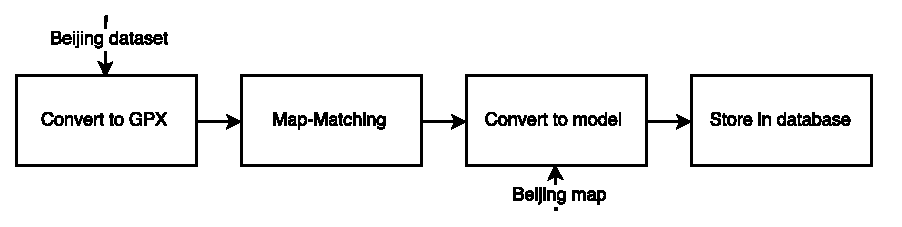
\includegraphics[width=1\textwidth]{figures/data-processing.pdf}
    \caption{From raw gps data to database}
    \label{fig:data-processing}
\end{figure}
The gps dataset is converted into the GPX format which is subsequently map-matched to the road network of Beijing. The map-matched data is then converted into the model objects of the system, and are then stored in the respective tables of the database. Likewise, the map of the Beijing road network is converted to model objects and stored in the database. By doing so, we have a knowledge base of the road network of Beijing and data about vehicle movements in a unified format. \todo{maybe we should perform some data cleaning}
\subsection{Map matching}
The Beijing dataset consists timestamped samples of gps-coordinates. The format of the samples is (id, date time, longitude, latitude). However since GPS measurements can be inaccurate, it is not always possible to directly infer which road the sample was taken on. Consequently the coordinates must be map-matched to a road, such that positions on the road can be inferred. To perform map-matching, the system calls the TrackMatching webservice\cite{TrackMatching}. This service exposes an API for map-matching to the OpenStreetMap service and given a dataset of raw GPS-coordinates returns a map-matched dataset in JSON format. 
\todo{write about how and why map generation}
\todo{write about how and why we design DB and store data in SQL database}
